\chapter{Introducción}
	
Este primer capítulo describe de forma general la información principal y relevante para poder comprender el funcionamiento del producto actual LUCA, así como los objetivos del proyecto a desarrollar junto con la explicación y motivación del mismo.
	
\section{Introducción}


Dado que el presente trabajo se enmarca dentro del proyecto LUCA, para poder comprender los objetivos de este Trabajo Fin de Grado, se hace necesario describir primero dicho proyecto, lo cual se realiza en la siguiente sección.

\section{LUCA}

\subsection{Motivación}

En los últimos años, el volumen de datos recogidos y manipulados por las empresas ha aumentado de forma vertiginosa. Estos datos se han ido almacenando en diferentes tipos de fuentes conforme las empresas crecían y sus sistemas evolucionaban y se fusionaban. Como resultado de  este proceso no es extraño actualmente encontrar empresas que tengan sus datos almacenados en sistemas tan dispares como bases de datos relacionales, hojas XML o repositorios FTP.


Como consecuencia de esta nueva situación, cuando un usuario quiere obtener una información concreta cuyos datos residen en varios de estos sistemas, éste necesita acceder a cada uno de estos sistemas, extraer de cada sistema la información que precisa, y finalmente filtrarla y unificarla para finalmente obtener los datos requeridos.

Por ejemplo, una cadena de venta de electrodomésticos podría tener sistemas informáticos diferentes para el departamento de atención al cliente, para el departamento técnico de postventa y para el departamento de compras y adquisiciones. Por tanto, para conocer con precisión el estado actual de una reparación, podríamos necesitar:

\begin{enumerate}
	\item Acceder al sistema de atención al cliente para obtener el identificador de la incidencia y en qué fase de su gestión se encuentra.
	\item Una vez corroborado que la incidencia está actualmente siendo atendida, recuperaríamos del sistema de gestión de reparaciones el estado detallado de la reparación. Como resultado de esta operación, supongamos que averiguamos que la reparación está a la espera de recibir una pieza que se ha de sustituir.
	\item Finalmente, para poder hacer una estimación de cuando podría estar lista la reparación, accederíamos al sistema de compra y adquisiciones para averiguar cuando está prevista la entrega de la pieza solicitada.
\end{enumerate}

Como hemos comentado anteriormente, a cada uno de estos sistemas podría accederse de manera diferente. Por ejemplo, el primero podría consultarse utilizando un servicio web. La información del segundo podría recuperarse accediendo directamente a una base de datos relacional, mientras que la información del tercero se obtendría analizando órdenes de compra en formato \emph{pdf} almacenadas en un repositorio de ficheros compartido. Por tanto, el usuario, para poder realizar este proceso, necesita conocer las particularidades de cada sistema y de su forma de acceso.

Para aliviar esta situación, dentro de la empresa CIC, se está desarrollando una aplicación denominada LUCA, a la cual contribuye este Trabajo Fin de Grado. Para facilitar este proceso de recuperación de información, LUCA proporciona un lenguaje común para todas las fuentes de datos a unificar, permitiendo al usuario abstraerse de los detalles de cada fuente.

\subsection{Funcionamiento de LUCA}

A continuación, se detalla brevemente el funcionamiento de \emph{LUCA}. Para ello, utilizaremos como ejemplo una consulta a la base de datos de LUCA, esta consulta obtendrá los procesos en función de un estado (los estados pueden ser en edición, publicado, es decir, preparada para ser ejecutada, o borrado). 

\begin{figure}[!tb]
    \centering
 	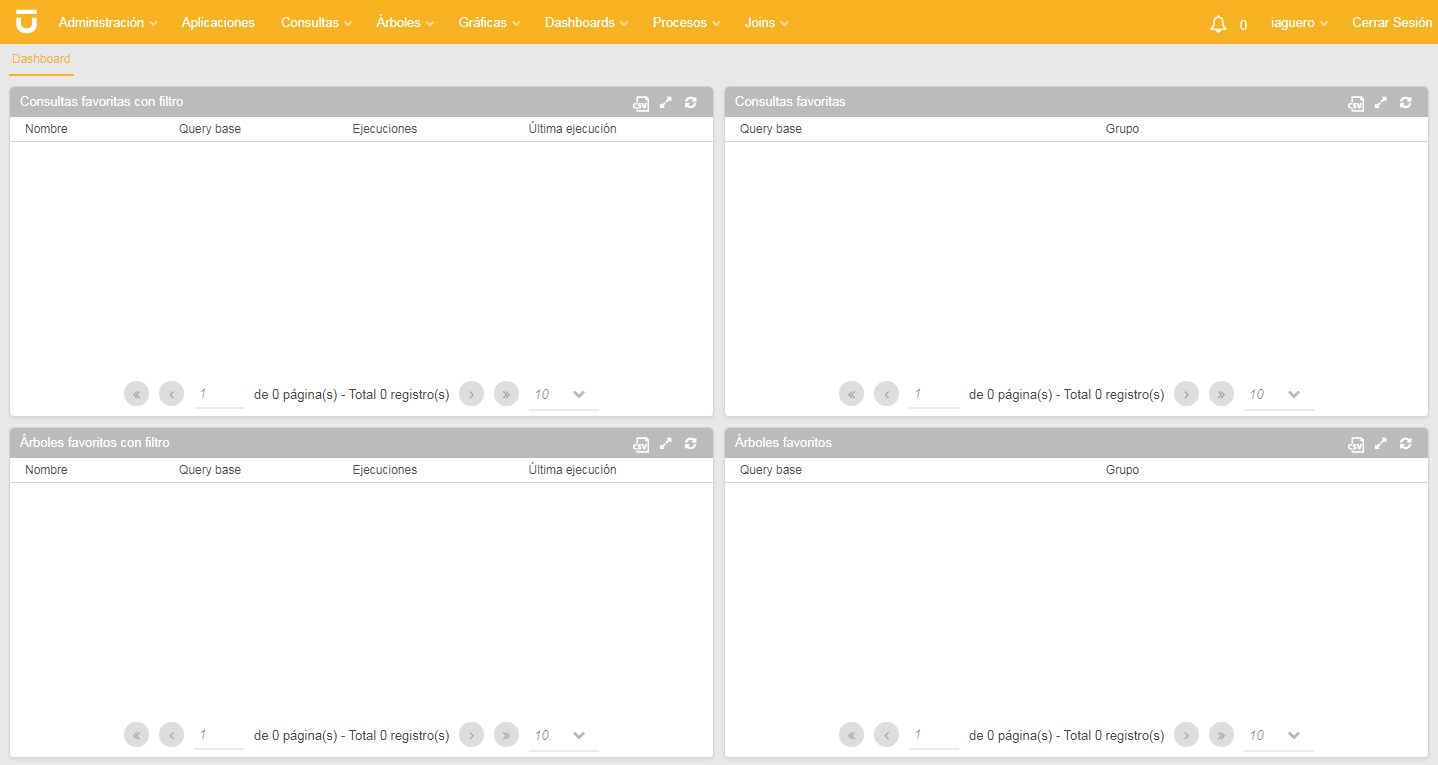
\includegraphics[width=\linewidth]{capturasLuca/menuLuca.png}
	\caption{Menu Principal LUCA}
    \label{fig:menuLuca}
\end{figure}

En el menu principal de LUCA, nos aparece una vista con un conjunto de consultas que el usuario ha marcado como favoritas (Figura~\ref{fig:menuLuca}), es decir, que suele utilizar con frecuencia. Como se dijo anteriormente, se utilizará la consulta de los procesos por estado.

\begin{figure}[!tb]
	\centering
	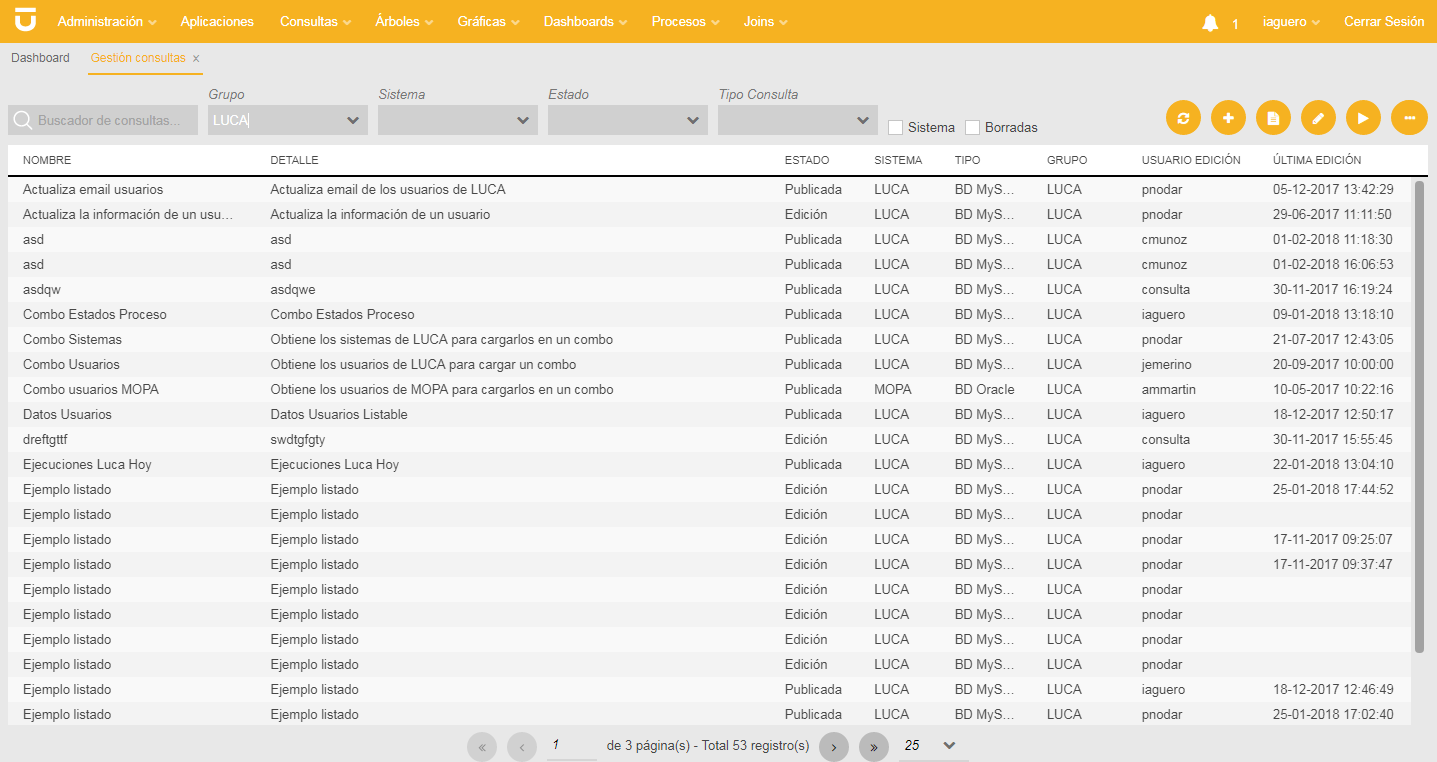
\includegraphics[width=\linewidth]{capturasLuca/gestionConsultas.png}
	\caption{Vista de Gestión de Consultas}
	\label{fig:gestionConsultas}
\end{figure}

En la vista de gestión de consultas (Figura~\ref{fig:gestionConsultas}) se pueden realizar las operaciones propias de la gestión, como es crear, modificar, eliminar o ejecutar entre otras.

No obstante, para que dichas consultas pueden ser ejecutadas, es necesario un usuario con conocimientos suficientes para ello, al que denominaremos en adelante el \emph{creador de consultas}.

\begin{figure}[!tb]
	\centering
	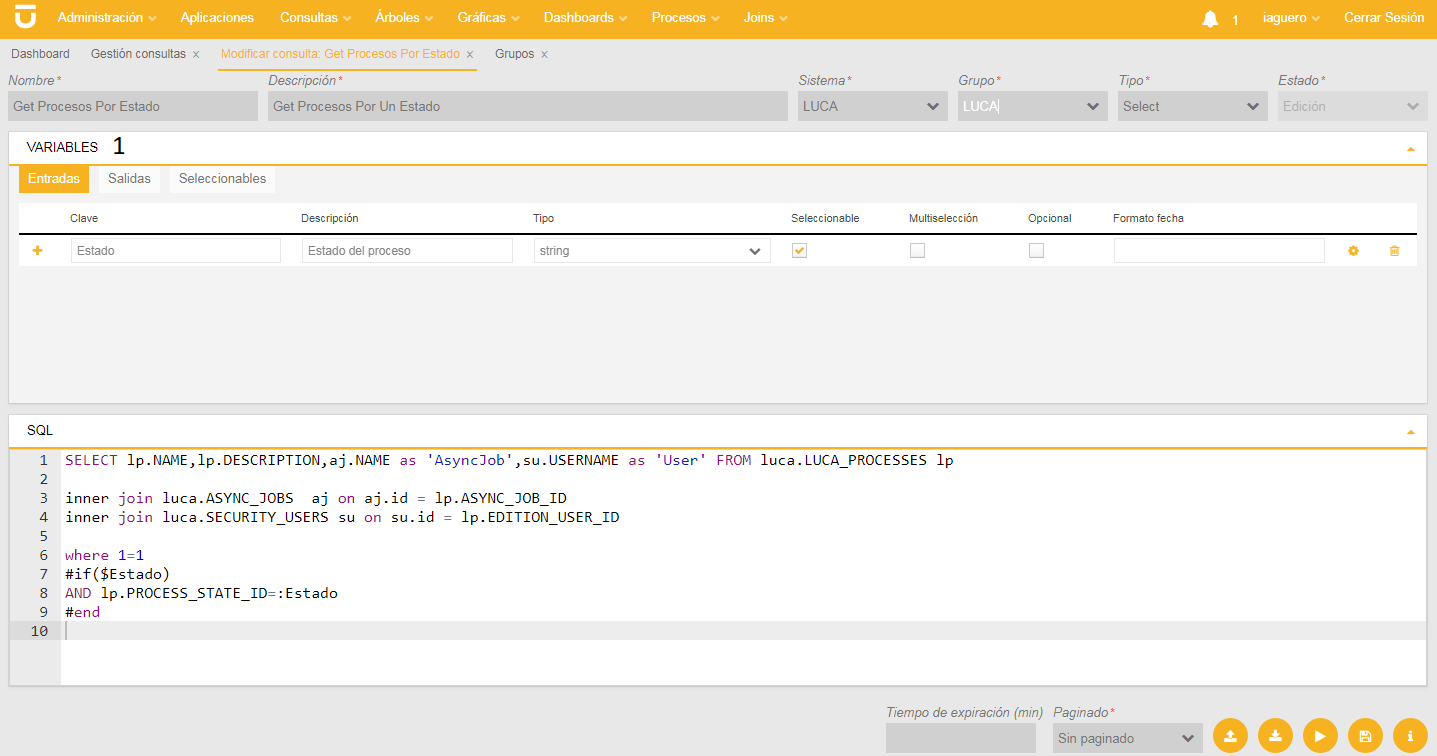
\includegraphics[width=\linewidth]{capturasLuca/creacionConsulta.png}
	\caption{Creación de una Consulta}
	\label{fig:creacionConsulta}
\end{figure}

Para poder realizar esta tarea, el creador de consultas accedería a la interfaz dedicada a esta tarea (ver Figura~\ref{fig:creacionConsulta}). En esta interfaz, definiría primero las variables de entrada y salida de la consulta (Figura~\ref{fig:creacionConsulta}, etiqueta 1). A continuación, especificaría cómo llevar a cabo dicha consulta a bajo nivel. Para ello puede utilizar una serie de facilidades y primitivas proporcionadas por LUCA. Para la consulta ejemplo, utilizando estas facilidades, se especifica que se desea obtener el nombre, la descripción, el nombre de la tarea asíncrona y el usuario, y se establece como variable de entrada el estado del proceso.

Tras guardar la consulta se puede ejecutar directamente desde la ventana de creación, sin embargo, si la consulta ya ha sido ejecutada previamente y el usuario la ha publicado (tras ejecutar una consulta desde la ventana de creación, si se ha ejecutado correctamente se le permite al usuario cambiar su estado de edición a publicada, esto significa que la consulta está preparada para ser ejecutada), el usuario puede ir a la ventada de ejecución de consultas, y desde ahí ejecutarla.

La principal ventaja que aporta LUCA es que el proceso de ejecución de consultas es opaco para el usuario que la ejecuta. El usuario sólo tiene que proporcionar los parámetros necesarios de entrada y seleccionar un formato de salida. Por tanto, el proceso de ejecución de consultas es exactamente el mismo con independencia de la fuente a la cual se accede.

Por ejemplo, en el caso de la consulta \emph{Get Procesos Por Estado} sería necesario proporcionar el estado de los procesos de los que queremos obtener información. Una vez introducido dicho estado, se seleccionaría el botón de ejecución de la consulta (Figura~\ref{fig:ejecucionConsulta}, etiqueta 2). Finalmente, se muestra el resultado de la consulta, el cuál puede ser visualizado de diferentes formas en función del recurso al que se llama. En nuestro caso, se muestra como una tabla ya que es una consulta a base de datos (Figura~\ref{fig:ejecucionConsulta}, etiqueta 3).

Lo importante de este proceso es que, una vez definida la consulta, ésta se puede ejecutar fácilmente sin conocer los detalles internos de la misma, incluso hasta el tipo de sistema al que se accede.


	\begin{figure}[!tb]
		\centering
		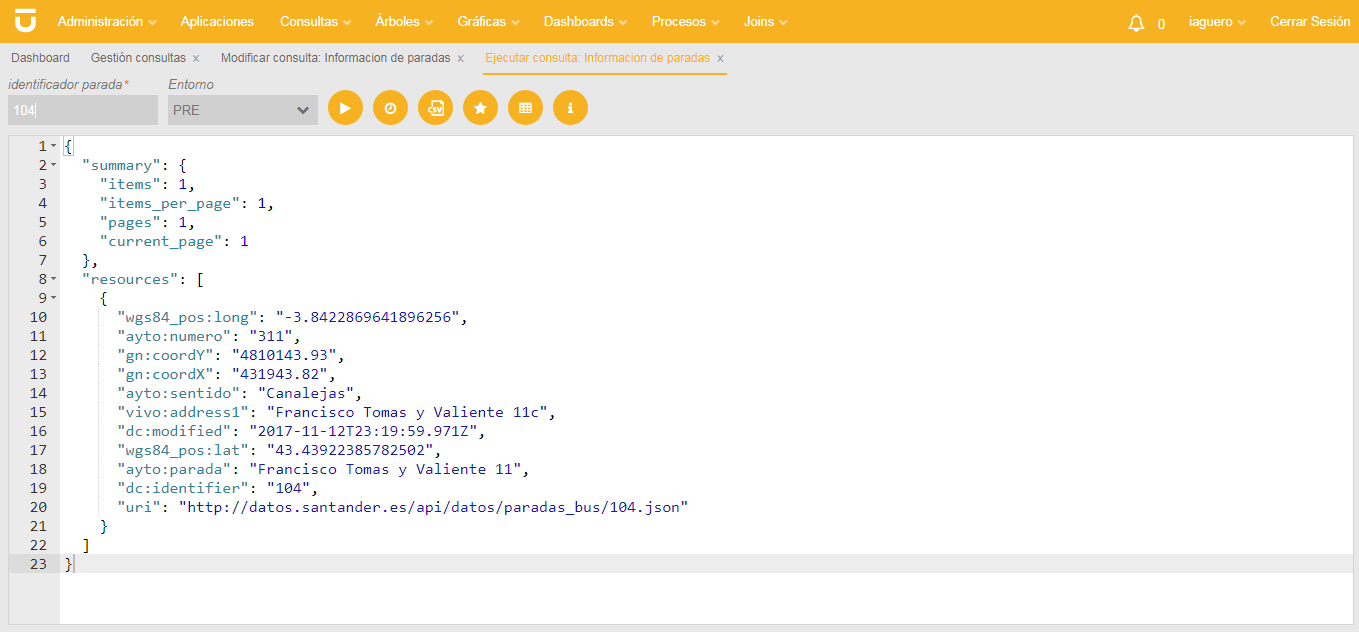
\includegraphics[width=\linewidth]{capturasLuca/ejecucionConsulta.png}
		\caption{Vista de Ejecución de Consultas}\label{fig:ejecucionConsultas}
	\end{figure}

\subsection{Limitaciones actuales de LUCA}

Actualmente, LUCA proporciona mecanismos para permitir al usuario recuperar de manera uniforme información de diferentes fuentes de datos. No obstante, LUCA por el momento sólo es capaz recuperar información de una única fuente de datos a la vez. Por tanto, cuando es necesario combinar información procedente de distintas fuentes, el propio usuario es el que debe realizar dicho proceso de composición a mano, ejecutando él cada consulta, y utilizando las salidas de cada una de ellas como entradas para las siguientes.


Un ejemplo de dicho proceso de composición sería la necesidad de un dependiente de una tienda de electrodomésticos de obtener la edad de los usuarios que compraron lavadoras durante el mes pasado. Actualmente, la secuencia de consultas que debería de realizar serían las siguientes:

\begin{itemize}
	\item Primero necesitaría obtener el registro de compras del mes pasado del sistema.
	\item Después, tras guardar dicho registro, tendría que, uno por uno, seleccionar los que se corresponden con lavadoras.
	\item Una vez que el usuario tiene las lavadoras compradas el mes pasado, éste tendría que extraer que usuarios han comprado las lavadoras.
	\item Por último, debería buscar en el sistema cada usuario que ha realizado la compra, a partir del nombre obtenido en el punto anterior, y anotar su edad.
\end{itemize}

En adelante, estas cadenas de consultas para obtener un resultado concreto las denominaremos \emph{procesos}. El problema actual de LUCA, tal como ilustra el ejemplo anterior, es que no soporta el concepto de \emph{proceso}. Por tanto, para ejecutar un proceso,  el usuario tiene que realizar una larga y compleja secuencia de acciones.

\section{Objetivos del Trabajo de Fin de Grado}

El objetivo general de este Trabajo Fin de Grado es integrar en LUCA el concepto de \emph{proceso}. Para ello, hay que dar soporte a dos cuestiones diferentes: (1) la ejecución de los procesos; y (2) la especificación de procesos. Por tanto, el objetivo general de este trabajo se descompone en estos dos subobjetivos principales. 

El primer objetivo implica poder tratar procesos en LUCA de la misma forma que se trata las consultas. Es decir, los procesos deberán aparecer como en las consultas bajo una pestaña de gestión y otra de ejecución. Obviamente, la complejidad de ejecutar una proceso es mayor que la de ejecutar una consulta, ya que necesitamos ejecutar varias consultas, guardar resultados intermedios y utilizar estos resultados como entradas para otras consultas.

El segundo objetivo, que es el que implica una mayor complejidad, consiste en facilitar la especificación de procesos en LUCA. Para que un proceso pueda ser ejecutado, primero debe ser especificado, indicando qué consultas lo componen y cómo se relacionan. De acuerdo con los deseos expresados por los responsables del proyecto LUCA y la empresa CIC, dicho mecanismo de especificación debía ser gráfico, permitiendo así componer consultas de manera visual mediante la interconexión de las salidas de unas con las entradas de otras.

Para refinar estos dos grandes objetivos en una serie de requisitos más concretos, se llevó a cabo en primer lugar una reunión con el Jefe y el Gerente del proyecto. El objetivo de dicha reunión era conocer LUCA en profundidad. A continuación, dado que la fase de Ingeniería de Requisitos para este proyecto ya había sido realizada por la propia empresa, se nos proporcionaron unos documentos técnicos con los requisitos técnicos tanto para la ejecución de procesos como para el desarrollo del componente gráfico de especificación de procesos. Estos documentos pueden encontrarse en el Anexo adjunto a la memoria.


Como ya se ha mencionado, en estos documentos se pueden encontrar los requisitos técnicos atribuidos al proyecto, pero, de forma resumida, se centran en tres pilares o requisitos principales:



\begin{itemize}
	\item Concatenación de las consultas entre si pertenecientes a un mismo proceso.
	\item Visualización del progreso de ejecución del proceso.
	\item Aplicar criterios de navegación a partir de los resultados de salidas.
\end{itemize}


\section{Arquitectura LUCA}

LUCA se basa en una arquitectura en tres capas utlizando el patrón \emph{Model-View-Presenter} o MVP\cite{mvp} (Figura \ref{fig:funcionamientoLuca}). Este patrón esta orientado a crear interfaces de usuario y su objetivo es separar la lógica de la aplicación. Además ayuda a realizar pruebas automatizadas de la interfaz gráfica. 

Se compone de tres módulos independientes entre si: modelo, vista y presentador. El modelo es el encargado de gestionar los datos que van a ser mostrados o no en la interfaz. La vista es una interfaz que se encarga de mostrar datos a partir de órdenes desde el presentador, y comunica al presentador sobre los eventos ocurridos en la interfaz. Por último el presentador es una capa situada entre el \emph{Modelo} y la \emph{Vista} y se encarga de conectar ambas, recuperando los datos del repositorio o fuentes de datos para posteriormente recargar la vista. Además, define las acciones a realizar cuando se producen eventos en la interfaz sobre los diferentes componentes de la vista.

Luca se beneficia de una arquitectura en capas independientes entre sí, que permite que la aplicación sea muy modular y escalable. Se compone de de tres capas: presentación, negocio y persistencia. A continuación se desglosa el funcionamiento de cada una:
\begin{itemize}
	\item Presentación \subitem Es la encargada de presentar los datos a la interfaz, además de comunicar los eventos ocurridos en la vista a la capa de negocio. Fijándonos en el patrón \emph{MVP} descrito anteriormente, esta capa se correspondería con las vistas.
	\item Negocio \subitem Esta capa se encarga de gestionar la lógica de la aplicación y se correspondería con el presentador en el patrón \emph{MVP}.
	\item Persistencia \subitem Esta capa se encarga de almacenar, obtener, modificar y eliminar los datos. En el patrón \emph{MVP} encaja con el Modelo, aunque esta capa tiene más características. En LUCA, esta capa se divide en tres subcapas inferiores. La capa  controladora, encargada mayoritariamente de la seguridad en el acceso a datos. La capa de servicio, encargada de acceder a las fuentes de información para obtener los datos. Y por último la capa de repositorio, encargada de acceder a la base de datos. La capa de servicio es la encargada de decidir el lugar de donde obtener los datos, por lo tanto, dependiendo de la naturaleza de la consulta, esta capa se comunicará con un \emph{Conector} (se explicará posteriormente) o con la base de datos.
\end{itemize}




\begin{figure}[!tb]
	\centering
	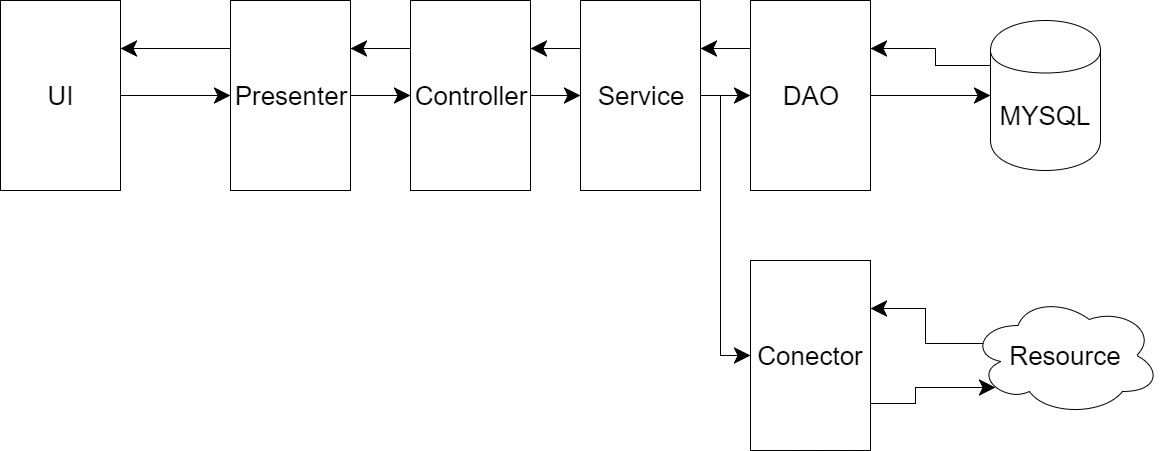
\includegraphics[width=\linewidth]{funcionamientoLuca.png}
	\caption{Arquitectura de LUCA}
    \label{fig:funcionamientoLuca}
\end{figure}



\subsection{Arquitectura del Conector}


El conector de LUCA es un componente que se encarga de recibir los datos de los diferentes recursos albergados en las diferentes fuentes de datos externas. En función del tipo de recurso con el que va a comunicarse, utilizará un tipo de conector u otro, ya sea el \emph{HTTPClient} \cite{httpclient} de \emph{Apache} o \emph{JDBC} \cite{jdbc} de \emph{Oracle}. En la figura \ref{fig:conectorImplementation} podemos ver un diagrama que describe dicha interacción.

Por ejemplo, si una consulta se realiza sobre un servicio \emph{REST}, cuando el presenter pida a la capa de servicios ejecutar una consulta, esta se comunicará con el conector \emph{HTTPClient} y no con la capa de repositorio, para poder realizar la consulta contra dicho servicio.

\begin{figure}[!tb]
	\centering
	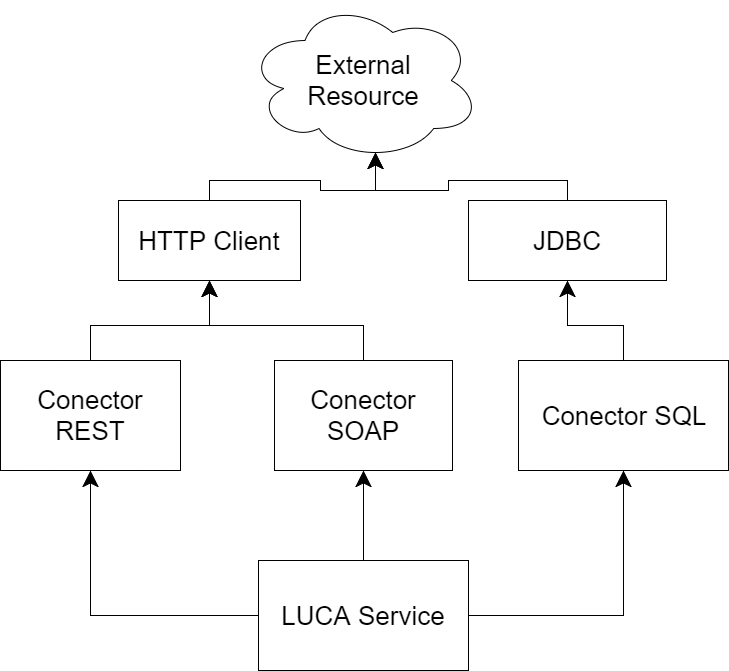
\includegraphics[width=\linewidth]{conectorImplementation.png}
	\caption{Arquitectura del Conector}\label{fig:conectorImplementation}
\end{figure}

\subsection{Arquitectura del Process-Component}

El Process-Component es un proyecto independiente a LUCA y que deberá de ser implementado. Su objetivo es fundamentalmente ejercer las labores de la vista, y se in componente encargado de mostrar elementos en pantalla. 

La arquitectura del Process-Component se ostenta en dos pilares. El primero la lógica de negocio del propio componente y el segundo es un fichero conector que se comunica con una librería de \emph{GO.JS} que también debe de ser definida.

Este componente se compone de un modelo de datos que deberá de ser implementado por cualquier proyecto que quiera usarlo. Su principal característica es poseer un conjunto de métodos encargados de crear, modificar y eliminar los diferentes elementos que serán plasmados en la vista. Este modelo será traducido a un conjunto de clases diseñadas específicamente para ser enviadas al \emph{Conector} para que este visualice los datos.


El \emph{Conector} internamente importa la librería gráfica \emph{GoJS} (será explicada en apartados posteriores) y se encargará insertar, modificar o eliminar los elementos del modelo de esta librería. Por lo tanto actuará de intermediario entre el modelo del \emph{Process-Component} y de \emph{GoJS}.

A continuación, se muestra una figura explicativa de dicha interacción interna entre los componentes:

\begin{figure}[!tb]
	\centering
	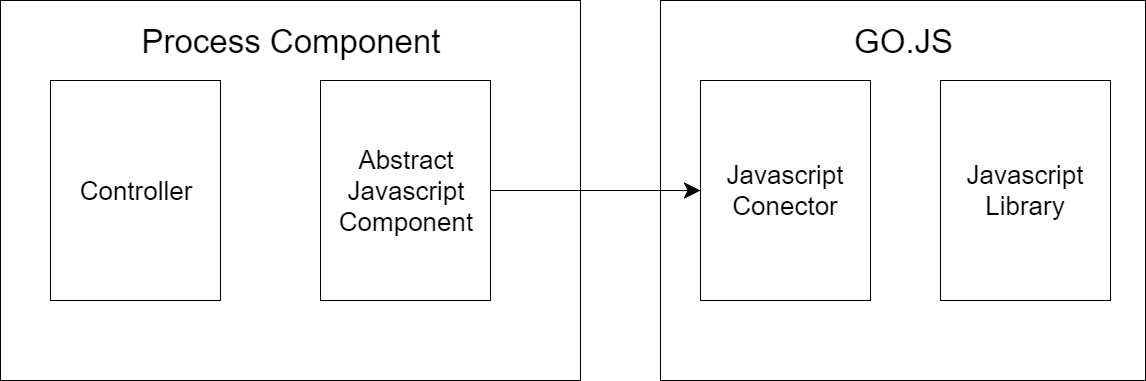
\includegraphics[width=\linewidth]{processComponentArquitectura.png}
	\caption{Arquitectura del Process-Component}\label{fig:processComponent}
\end{figure}

Como resumen del funcionamiento del Process-Component, éste es el encargado de recibir eventos realizados sobre la interfaz gráfica, a través del conector hasta llegar a la lógica del componente donde se tratarán y de realizar modificaciones sobre la vista.

	
\subsection{Pruebas}
	
	
	Las pruebas se centraron principalmente en el Luca-Process, ya que es el componente que alberga la mayor lógica del proyecto debido al conjunto de servicios que lo compone y a la lógica sobre los presenters desplegada.
	
	
	Profundizando en las pruebas implementadas, solo se han realizado pruebas de integración por varios motivos. El primero es que las pruebas unitarias no son necesarias hacerlas ya que se centran sobre la capa de repositorio y esta capa ha sido implementada con Spring Data Jpa\cite{jpa} y ofrece ya una fiabilidad. El motivo por el que no se realizaron pruebas de sistema, aunque en una primera planificación estaban previstas hacerlas integrandolas con Selenium\cite{selenium} fue la complejidad que lleva la integración junto con Vaadin\cite{vaadin}, ya que la ventaja de programar mediante una captura de eventos sobre la vista toda la secuencia de movimiento sobre dicha vista pasa a ser programática, y debido a que había que ceñirse a unas fechas de entrega y al tiempo que llevaría dicha implementación se decidió omitirlas.

	
	Las pruebas de integración que se llevaron a cabo se implementaron con Spring Test\cite{springTest} y JUnit\cite{junit}. Desglosando la composición de los mismos, se utilizó en cada test un fichero sql que declaraba las instrucciones de inserción de datos en la base de datos de pruebas necesarios para el correcto funcionamiento de los mismos. La base de datos de pruebas es una base de datos Mysql en local. relacional





	 